\documentclass[11pt]{article}
%more features in math mode
\usepackage{amsmath}


%for "here"
\usepackage{float}

%mathcal and stuff
\usepackage{amsfonts}

%seems to not work if removed
\usepackage{amsrefs}

%theorems
\usepackage{amsthm}

%commutative diagrams
\usepackage{tikz-cd}

%draw polygons
\usepackage{tikz}

%include pictures
\usepackage{graphicx}

%subfigures
\usepackage{caption}
\usepackage{subcaption}

%french spacing
\frenchspacing



\title{Pretzel Knots Have Coxeter Quotients}
\date{16. March 2019}

\newtheorem{theorem}{Theorem}[section]
\newtheorem{proposition}[theorem]{Proposition}
\newtheorem{lemma}[theorem]{Lemma}
\newtheorem{corollary}[theorem]{Corollary}
\newtheorem{conjecture}[theorem]{Conjecture}
\theoremstyle{definition}
\newtheorem{definition}[theorem]{Definition}
\newtheorem{example}[theorem]{Example}
\newtheorem{remark}[theorem]{Remark}
\newtheorem{notation}[theorem]{Notation}

\begin{document}
\section{The Word Problem for Coxeter Groups}

To show that the fundamental groups of pretzel link complements have Coxeter quotients (Theorem \ref{thm:pretzel-coxeter}) that are in some sense unique, we first consider a particular solution of the word problem for Coxeter groups (Proposition \ref{prop:word-problem-coxeter}). But first, we need to agree on some

\begin{notation}\label{not:coxeter-groups}
Suppose we are given a finite set $S = \{s_1, \dots, s_n\}$ for $n \geq 2$ and a symmetric matrix $M = (m_{ij})$ of size $n \times n$, where the $m_{ij}$ are natural numbers or $\infty$ such that for $i \neq j$ we have $m_{ij} \geq 2$,
and for all $i$ we have
$m_{ii} = 1.$
Then $W$ is the Coxeter group presented as
$$W = \langle s_1, \dots, s_n \; | \; (s_is_j)^{m_{ij}} \text{ for } i, j = 1, \dots, n \rangle.$$
Moreover, we agree on the convention that
$$(s_is_j)^{m_{ij}/2} =  \begin{cases}
(s_is_j)^k & \text{ if } m_{ij} = 2k, \\
(s_is_j)^ls_i & \text{ if } m_{ij} = 2l + 1.
\end{cases}$$
E.g., if $m_{ij}=5$ we write $(s_is_j)^{5/2} = s_is_js_is_js_i$. 
\end{notation}

Now the solution of the word problem for $W$ can be found in Cohen's script, Theorem 4.3.1. Here is a formulation.

\begin{proposition}[The Word Problem for Coxeter Groups]\label{prop:word-problem-coxeter}
Let $M$ be the free monoid generated by $s_1, \dots, s_n$. Suppose the word $w \in M$ represents the trivial element in $W$. Then there is a sequence of moves of the following two types carrying $w$ to the empty word $\varepsilon \in M$.
\begin{center}
\begin{tabular}{c c c c}
\textup{(}i\textup{)} & $(s_i)^2$ & $\leadsto$ & $\varepsilon$ \\
\textup{(}ii\textup{)} & $(s_is_j)^{m_{ij}/2}$ & $\leadsto$ & $(s_js_i)^{m_{ij}/2}$ \\
\end{tabular}
\end{center}
\end{proposition}

\begin{lemma}\label{lem:divisors}
If $(s_js_i)^l = (s_ks_j)^m$, where $i,j,k$ are pairwise distinct, then we have that $m_{ij}$ divides $l$ and $m_{jk}$ divides $m$.
\end{lemma}

\begin{proof}
We will use the moves (\textit{i}) and (\textit{ii}) from Proposition \ref{prop:word-problem-coxeter}. Let
$$w = (s_is_j)^l(s_ks_j)^m.$$
We want to show that $w$ is trivial in $W$. By removing occurences of $(s_js_i)^{m_{ij}}$ and $(s_ks_j)^{m_{jk}}$ we can assume that $l < m_{ij}$ and $m < m_{jk}$. If $l \geq m_{ij}/2$, using move (\textit{ii}) on $(s_is_j)^l$ and afterwards applying move (\textit{i}) successively replaces the word $(s_is_j)^l$ by $(s_is_j)^{m_{ij}-l}$. So we can even assume that $l < m_{ij}/2$. Similarly, we can arrange $m < m_{jk}/2$. But then there are no more moves to apply that can decrease the number of occurences of $s_i$ or of $s_k$. But this implies that $l=m=0$ after iteratively subtracting $m_{ij}$ and $m_{jk}$, respectively.
\end{proof}

\section{Coxeter Quotients of Pretzel Link Groups}\label{sec:coxeter-quotients}

\begin{definition}
Let $K$ be a link and $G = \pi_1(S^3 \setminus K)$. Then we say that the Coxeter group
$W$ is an \textit{$S$-maximal Coxeter quotient} of $G$ if $W$ is a Coxeter quotient of $G$ with generating set~$S$, and any other Coxeter quotient of $G$ with generating set $S$ is isomorphic to a quotient of $W$.
\end{definition}


\begin{theorem}[Coxeter Quotients of Pretzel Link Groups]\label{thm:pretzel-coxeter}
Let $K\subset S^3$ be a pretzel link. Let $S = \{s_1,\dots,s_n\}$, where the $s_i$ are the meridians indicated in Figure \ref{fig:pretzel-meridians}. Then there is a unique $S$-maximal Coxeter quotient of~$\pi_1(S^3 \setminus K)$.
\end{theorem}

\begin{figure}
\center{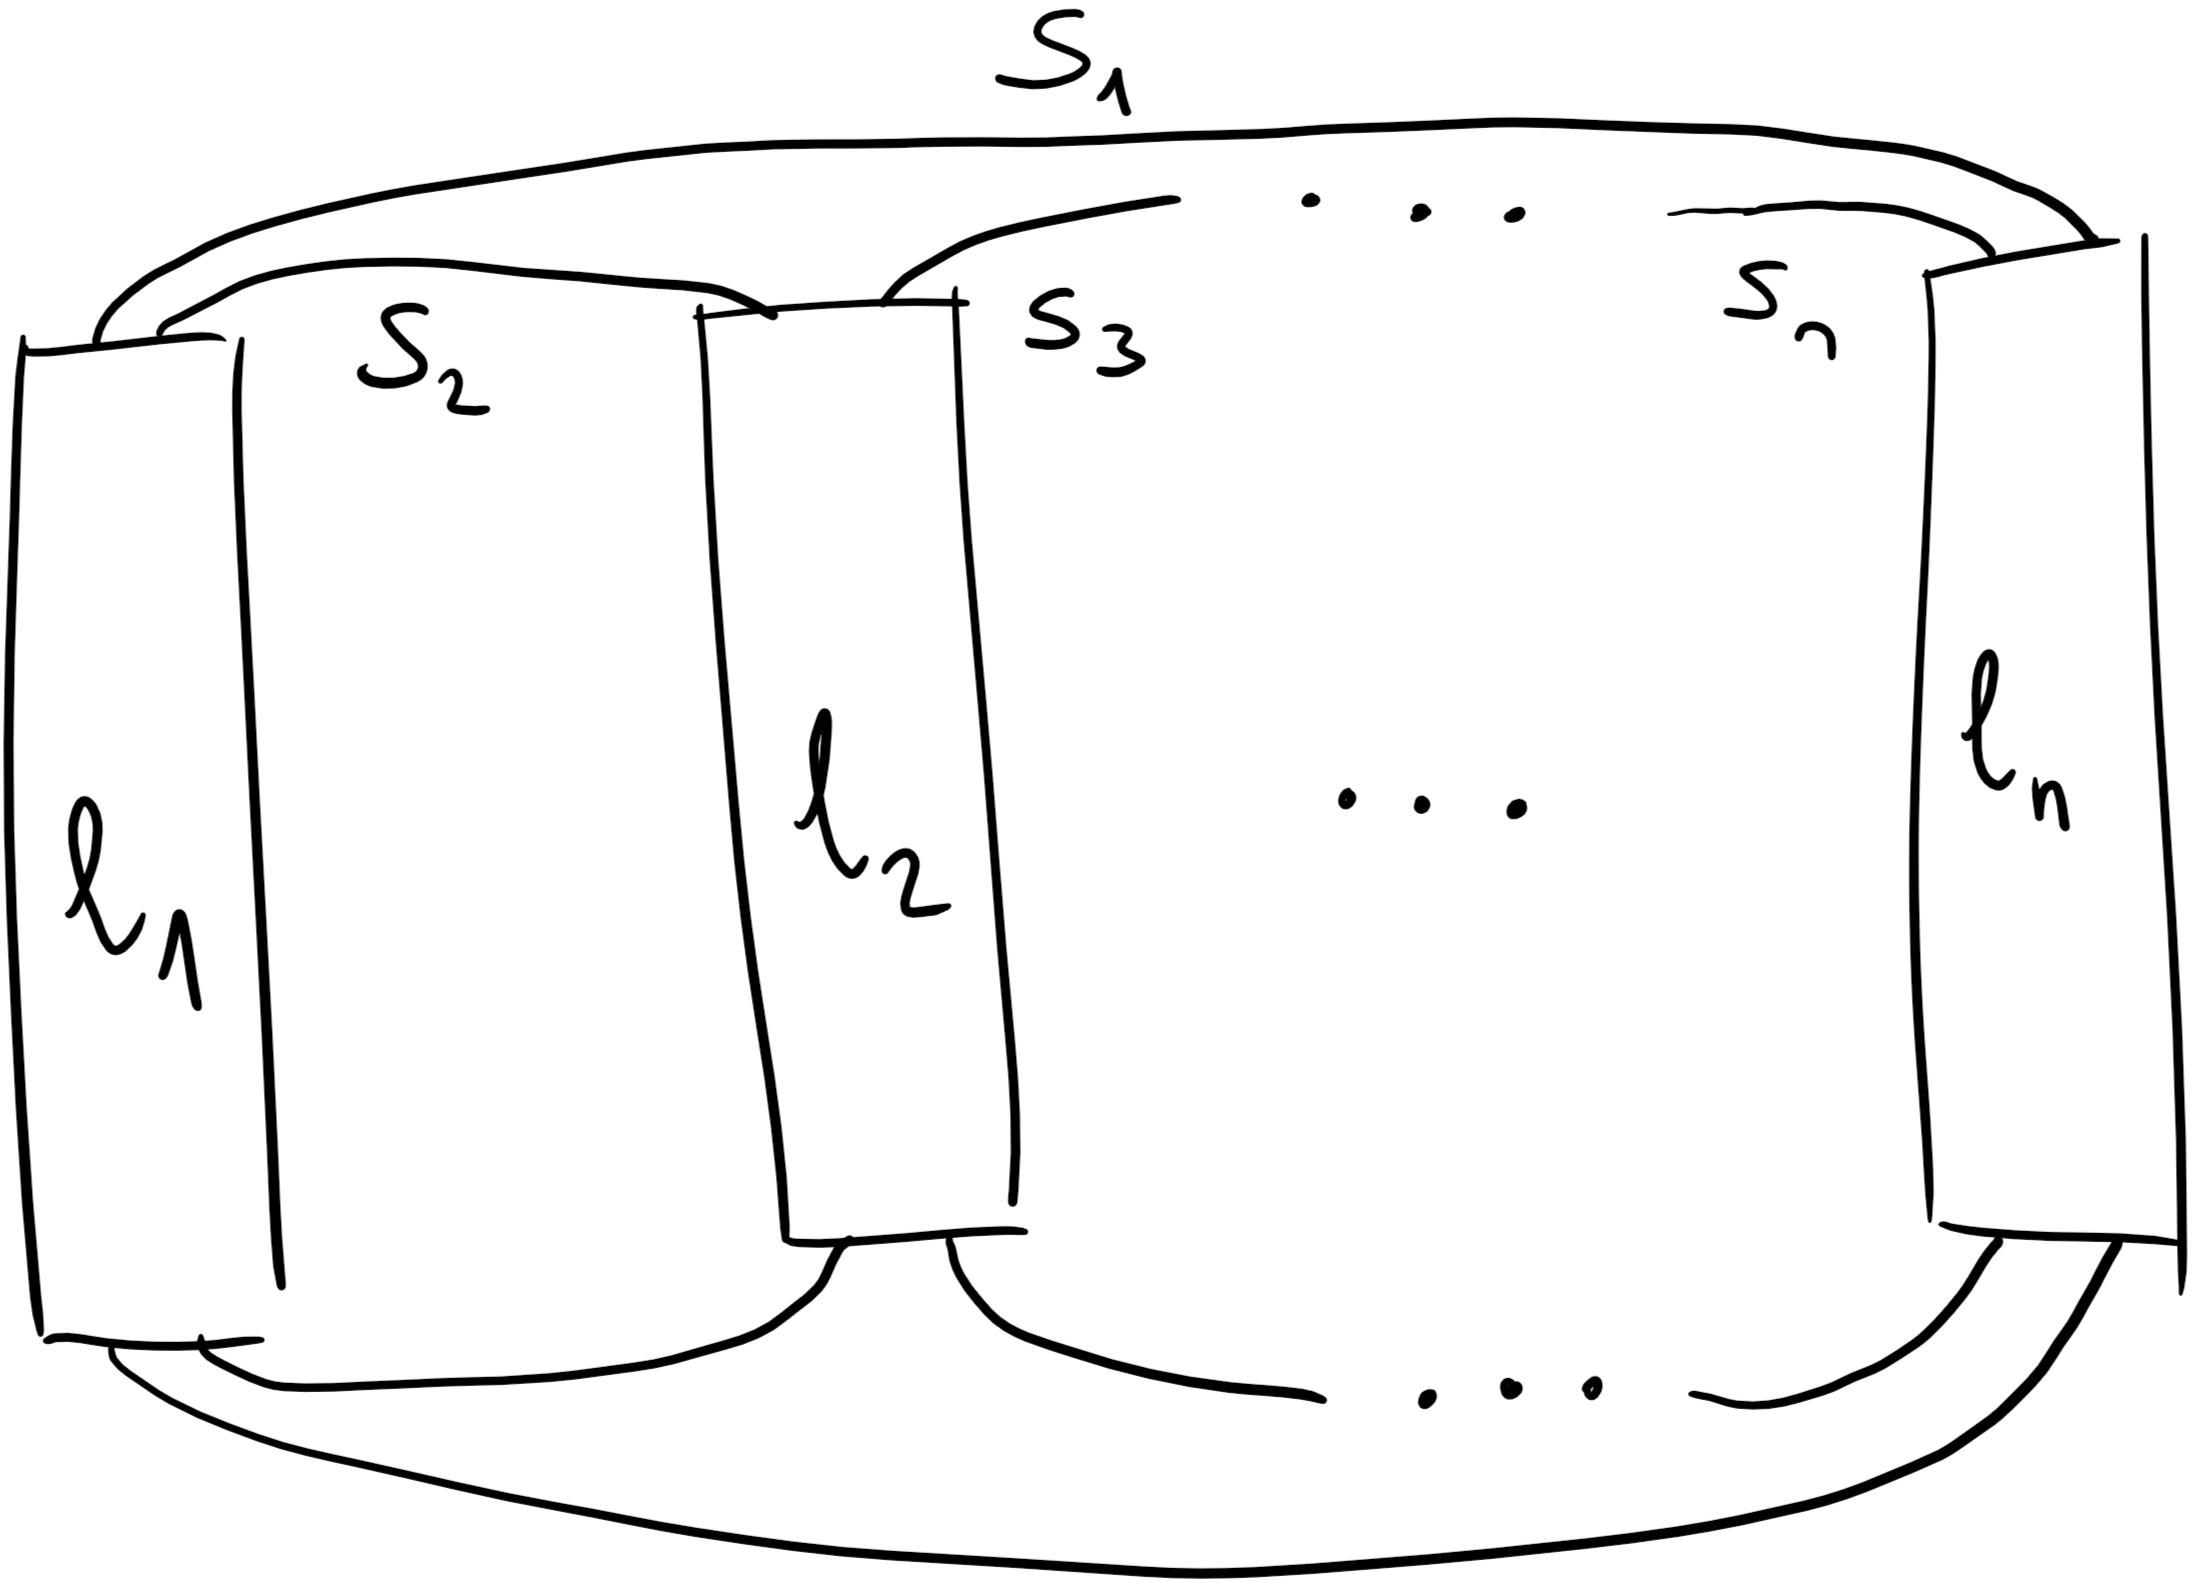
\includegraphics[scale = 0.22]
{figures/pretzel.png}}
\caption{\label{fig:pretzel-meridians} The generators of $\pi_1(S^3 \setminus K)$}
\end{figure}

\begin{proof}
By applying the Wirtinger algorithm and postulating $s^2 = e$ for all generators $s\in S$, one just gets the relations
$$(s_2s_1)^{l_1} = (s_3s_2)^{l_2} = \dots = (s_ns_{n-1})^{l_{n-1}}= (s_1s_n)^{l_n}.$$
By Lemma \ref{lem:divisors}, precisely those Coxeter groups generated by $S$ with $m_{i(i+1)}$ a divisor of $l_i$ satisfy these relations. Now let
$$M = \left( \begin{matrix}
1 & l_1 & \infty & \infty & \infty &\cdots & \infty & l_n \\
l_1 & 1 & l_2 & \infty & \infty & \cdots & \infty & \infty \\
\infty & l_2 & 1 & l_3 & \infty &\cdots & \infty & \infty \\
\infty & \infty  & l_3 & 1 & \ddots & \ddots & \vdots & \vdots \\
\infty & \infty & \infty & \ddots & \ddots & \ddots & \infty & \infty \\
\vdots & \vdots & \vdots & \ddots &\ddots & 1 & \l_{n-2} & \infty \\
\infty & \infty & \infty & \cdots & \infty & l_{n-2} & 1 & l_{n-1} \\
l_n & \infty & \infty & \cdots & \infty & \infty  & l_{n-1} & 1
\end{matrix} \right).$$
Then the Coxeter quotient $W$ corresponding to $M$ is $S$-maximal.
\end{proof}

\section{Bipolarity of Pretzel Coxeter Groups}

\begin{definition}
A Coxeter group $W$ is called \textit{spherical} if it is finite. Likewise, a generating set $S$ is called \textit{spherical} if $\langle S \rangle$ is finite. A Coxeter group is called \textit{irreducible} if its Coxeter graph, with the convention that an edge labeled $2$ is not an edge, is connected. An \textit{odd component} is a component of the graph whose vertices are $S$ and whose edges are the edges of the Coxeter graph with odd weights. For a subset $T\subset S$ we let $T^\perp$ be the subset of $S$ consisting of all the $s \in S$ that commute with all $t \in T$.
\end{definition}


\begin{proposition}\label{prop:coxeter-quotient-bipolar}
Let $K$ be a pretzel link with $n \geq 4$ braids, and let $S$ be the standard generating set indicated in Figure \ref{fig:pretzel-meridians}, and let $W$ be the $S$-maximal Coxeter quotient of the link group $\pi_1(S^3 \setminus K)$. Then $W$ is bipolar.
\end{proposition}

\begin{proof}
Let $\Gamma$ be the graph with vertices $S$ and an edge between $s_i$ and $s_j$ if $m_{ij}$ is finite. By Theorem 1.2 in Caprace-Przytycki it suffices to show the following three things.
\begin{enumerate}
\item There is no spherical irreducible component of $\Gamma$.
\item  There are no subsets $I \subset T$ with $T$ irreducible and $I$ non-empty spherical such that the subgraph induced by $I \cup T^\perp$ separates $\Gamma$.
\item If $T \subset S$ is irreducible spherical and an odd component $O$ of $S$ is contained in $T^\perp$, then there are adjacent $t\in O$ and $t' \in S\setminus (T \cup T^\perp)$.
\end{enumerate}

First we consider 1. The graph $\Gamma$ in question is $A_n$. This graph is connected so we just need to make sure that $W$ is not spherical irreducible. But this follows from the presence of infinite weights, which is guaranteed by the requirement that $n \geq 4$.

For statement 2., let $T \subset S$ be irreducible. We now distinguish a few cases. If $T = \{t\}$, then $I \cup T^\perp$ consists either of just $t$, or of two or three adjacent vertices in $\Gamma$, in all cases their complement in $\Gamma$ is connected. If we have $T = \{s,t\}$, then $T^\perp$ consists of at most one vertex adjacent in $\Gamma$ to both vertices $s$ and $t$, so we ultimately are in the same situations as in the previous case. Moreover, if $|T| \geq 3$, then $T^\perp$ is empty, and $I$ has at most two elements, which cannot separate $S$ since $n \geq 4$ and the two elements are adjacent in $\Gamma$.

Finally, for 3., if $T = \{t\}$ then $T^\perp$ is either empty, one or two non-adjacent vertices in $\Gamma$. In each case, $O$ does not exist or is one point. In case such an $O$ does exist, one can find such a $t'$ because $n\geq 4$. Whenever $|T| \geq 2$ we have that $T^\perp$ is empty, so there is no such $O$. This exhausts all the possibilities.
\end{proof}

\section{Maximal Quotients for Fixed Generating Set}
The existence of an $S$-maximal Coxeter quotient of Pretzel links, as shown in Theorem \ref{thm:pretzel-coxeter}, is an instance of the following more general phenomenon.

Fix a finite generating set $S$ of size $n$. Let $M = (m_{ij})$ and $M' = (m_{ij}')$ be Coxeter matrices. We say that $M$ \textit{divides} $N$ if $m_{ij}$ divides $m_{ij}'$ for all~$i,j$. This defines a partial order on the set $\mathcal{M}_S$ of Coxeter matrices with generating set $S$, with respect to which every subset has a join, namely
$$\bigvee_{k} (m_{ij}^{(k)}) = \left( \text{lcm}(m_{ij}^{(1)}, m_{ij}^{(2)}, \dots) \right).$$
The following Proposition summarizes our situation.

\begin{proposition}
The set $\mathcal{M}_n$ of Coxeter matrices of size $n$ equipped with the partial order 'divides' is a complete join-semilattice.
\end{proposition}

This gives us a convenient way to construct the $S$-maximal Coxeter quotient, as we will see in the proof of Theorem \ref{thm:general-s-maximal-quotients}. But first, we need a Lemma.

\begin{lemma}\label{lem:intersection-normal-subgroups}
Let $M^{(k)} = (m_{ij}^{(k)})$ be Coxeter matrices and let $N^{(k)}$ be the normal subgroup generated by the set of Coxeter relations corresponding to~$M^{(k)}$. Then
$$\bigcap_k N^{(k)} = N$$
where $N$ is the normal subgroup generated by the set of Coxeter relations corresponding to $M = \bigvee_k M^{(k)}$.
\end{lemma}

\begin{proof}
Obviously $N \subset N^{(k)}$ for all $k$, so we only need to show the other inclusion. Suppose $r \in N^{(k)}$ for all $k$. First consider the case $n = 2$, i.e., the groups corresponding to $M^{(k)}$ are dihedral groups. In this case the group generated by $R^{(k)}$ is cyclic. Proceed by induction.
%TODO
\end{proof}

\begin{theorem}[$S$-Maximal Quotients]\label{thm:general-s-maximal-quotients}
If a link $L \subset S^3$ has a Coxeter quotient of size $n$ with generating meridians $S = \{s_1, \dots, s_n\}$, then it has a unique $S$-maximal Coxeter quotient.
\end{theorem}

\begin{proof}
Let $M = \bigvee \mathcal{M}_{L,S}$ where $\mathcal{M}_{L,S}$ is the set of Coxeter matrices yielding Coxeter quotients of $\pi_1(S^3 \setminus L)$ with generating meridians $S$. If $R$ are the Wirtinger relations of $L$ with respect to $S$, then $R \subset N^{(k)}$ for each normal subgroup $N^{(k)}$ generated by the set of relations corresponding to some matrix $M^{(k)} \in \mathcal{M}_{L,S}$. Thus, by Lemma \ref{lem:intersection-normal-subgroups}, we also have $R \subset N$, where $N$ is the normal subgroup generated by the relations corresponding to $M$.
\end{proof}

\end{document}
